\documentclass[professionalfonts,compress,unicode,aspectratio=169]{beamer}
\usetheme{Moscow}

\usepackage[utf8]{inputenc}
\usepackage[T2A]{fontenc}
\usepackage[main=russian,english]{babel}

\usepackage{amsmath,amssymb}

\renewcommand{\thefootnote}{\fnsymbol{footnote}}
\hypersetup{pdfauthor={Ivan Tsybulin}}

\newcommand{\cutefrac}[2]{{}^{#1}\mkern-5mu/{\!}_#2}
\newcommand{\half}{{\cutefrac{1}{2}}}

\renewcommand{\thefootnote}{\fnsymbol{footnote}}

\graphicspath{{images//}}

\title[Краевая задача]{Краевая задача для ОДУ\\ Жесткая краевая задача}
\author[Цыбулин И.В.]{Скалько Юрий Иванович\\
\textbf{Цыбулин Иван}
}
\date{}

\newcommand{\colorhref}[2]{\href{#1}{\textcolor{miptbase!30!black}{#2}}}

\begin{document}

\begin{frame}[plain]
\titlepage
\end{frame}

\def\L{\mathcal{L}}

\section{Линейная краевая задача}
\subsection{Краевая задача для системы ОДУ}
\begin{frame}\frametitle{Краевая задача для системы ОДУ}
	В отличие от задачи Коши, условия, позволяющие зафиксировать конкретное
	решение уравнения ставятся на обоих концах отрезка:
	\[
	\begin{cases}
	\dfrac{d\mathbf{y}(x)}{dx} = \mathbf{G}(x, \mathbf{y}(x)), \qquad x \in [a,b]\\
	f_i(\mathbf{y}(a)) = 0, \quad i = 1, 2, \dots, r\\
	f_i(\mathbf{y}(b)) = 0, \quad i = r+1, r+2, \dots, n
	\end{cases}
	\]
	Требуется найти решение $\mathbf{y}(x)$ при $x \in [a, b]$
\end{frame}

\begin{frame}\frametitle{Линейная краевая задача для системы}
	В линейном случае правая часть системы представляется в виде
	\[\mathbf{G}(x, \mathbf{y}(x)) = \mathbf{A}(x) \mathbf{y}(x) +
	\mathbf{f}(x),\]
	а краевые условия --- в виде
	\[
	f_i(\mathbf{y}) = \boldsymbol{\ell}_i^\mathsf{T} \mathbf{y} - \alpha_i = 0
	\]
	\[
	\begin{cases}
	\dfrac{d\mathbf{y}(x)}{dx} = \mathbf{A}(x) \mathbf{y}(x) + \mathbf{f}(x), \qquad x \in [a,b]\\
	\boldsymbol{\ell}_i^\mathsf{T} \mathbf{y}(a) = \alpha_i, \quad i = 1, 2, \dots, r\\
	\boldsymbol{\ell}_i^\mathsf{T} \mathbf{y}(b) = \alpha_i, \quad i = r+1, r+2, \dots, n
	\end{cases}
	\]
\end{frame}

\subsection{Построение общего решения}
\begin{frame}\frametitle{Общее решение}
	Линейность уравнения позволяет искать решение в виде суммы частного решения неоднородной
	задачи и общего решения однородной.
	\[
	\mathbf{y}(x) = \mathbf{y}_\text{частн}(x) + \sum_{k=1}^n C_k \mathbf{y}_k(x)
	\]
	Здесь $\mathbf{y}_\text{частн}$ --- частное решение неоднородного уравнения,
	$\mathbf{y}_k$ --- $k$-е решение однородного уравнения.
\end{frame}

\begin{frame}\frametitle{Сведение к задачам Коши}
	Для численного построения $\mathbf{y}_i$ можно численно решать \emph{задачи Коши}.
	\[
	\begin{cases}
	\mathbf{y}_i'(x) = \mathbf{A}(x) \mathbf{y}_i(x)\\
	\mathbf{y}_i(0) = \mathbf{e}_i = (0, \dots, 0, 1, 0, \dots, 0)^\mathsf{T}
	\end{cases}
	\]
	$n$ таких решений образуют линейно независимую систему решений однородной
	системы. Для определения частного решения также численно решим задачу Коши с нулевыми
	начальными условиями:
	\[
	\begin{cases}
	\mathbf{y}_\text{частн}'(x) = \mathbf{A}(x) \mathbf{y}_\text{частн}(x) +
	\mathbf{f}(x)\\
	\mathbf{y}_\text{частн}(0) = 0
	\end{cases}
	\]
\end{frame}

\begin{frame}\frametitle{Нахождение нужного решения}
	Теперь у нас есть общее решение, которое можно составить из уже известных
	сеточных функций $\mathbf{y}_i, \mathbf{y}_\text{частн}$:
	\[
	\mathbf{y}(x) = \sum_{k = 1}^n C_k \mathbf{y}_k + \mathbf{y}_\text{частн}
	\]
	Подставляя это решение в краевые условия
	\begin{align*}
	&\boldsymbol{\ell}_i^\mathsf{T} \mathbf{y}(a) = \alpha_i, \quad i = 1, 2, \dots, r\\
	&\boldsymbol{\ell}_i^\mathsf{T} \mathbf{y}(b) = \alpha_i, \quad i = r+1, r+2, \dots, n
	\end{align*}
	получаем систему из $n$ линейных уравнений на $n$ неизвестных $C_k$. После
	определения $C_k$ решение получается из верхней формулы.
\end{frame}

\begin{frame}\frametitle{Эффективное построение общего решения}
	Ранее мы строили общее решение, игнорируя краевые условия полностью. При
	этом общее решение содержало $n$ констант и требовало решения $n+1$ задачи
	Коши.

	Покажем, как можно обойтись меньшим количеством.
	Рассмотрим задачу
	\begin{align*}
	&\mathbf{y}'(x) = \mathbf{A}(x) \mathbf{y}(x) + \mathbf{f}(x), \qquad x \in
	[0,1]\\
	&L_{i}^{-} \mathbf{y}(0) = \alpha_i^{-}, \quad i = 1,2\\
	&L_{i}^{+} \mathbf{y}(1) = \alpha_i^{+}, \quad i = 3,4,5
	\end{align*}
	где
	\begin{gather*}
	L^{-} = 
	\begin{pmatrix}
	0 & 1 & 2 & 0 & 1\\
	0 & 0 & 0 & 0 & 1
	\end{pmatrix}
	\quad
	\alpha^{-} = \begin{pmatrix} 1 \\ 2 \end{pmatrix}\\
	L^{+} = 
	\begin{pmatrix}
	0 & 0 & 1 & 0 & 1\\
	1 & 0 & 0 & 0 & 1\\
	0 & 0 & 0 & 1 & 1
	\end{pmatrix}
	\quad
	\alpha^{+} = \begin{pmatrix} 1 \\ 2 \\ 3\end{pmatrix}
	\end{gather*}
\end{frame}

\begin{frame}\frametitle{Решение, удовлетворяющее условиям на одной из границ}
	Найдем решение $\mathbf{y}(1)$ из системы (полужирным выделены базисные
	столбцы)
	\[
	\begin{pmatrix}
	\mathbf{0} & 0 & \mathbf{1} & \mathbf{0} & 1\\
	\mathbf{1} & 0 & \mathbf{0} & \mathbf{0} & 1\\
	\mathbf{0} & 0 & \mathbf{0} & \mathbf{1} & 1
	\end{pmatrix}
	\mathbf{y}(1) = 
	\begin{pmatrix} 1 \\ 2 \\ 3\end{pmatrix}
	\]
	Решение будет содержать две константы, поскольку система имеет ранг 3, а
	неизвестных в ней 5.
	\[
	\mathbf{y}(1) = 
	\begin{pmatrix}
	2 \\ 0 \\ 1 \\ 3 \\ 0
	\end{pmatrix}
	+ C_1
	\begin{pmatrix}
	0 \\ 1 \\ 0 \\ 0 \\ 0
	\end{pmatrix}
	+ C_2
	\begin{pmatrix}
	1 \\ 1 \\ 1 \\ 1 \\ -1
	\end{pmatrix}
	\]
	Заметим, что если находить решение системы для $\mathbf{y}(0)$, то
	неизвестных констант будет 3 (ранг системы равен 2).
\end{frame}

\begin{frame}\frametitle{Сведение к задачам Коши}
	Теперь, когда $\mathbf{y}(1)$ найден
	\[
	\mathbf{y}(1) = 
	\begin{pmatrix}
	2 \\ 0 \\ 1 \\ 3 \\ 0
	\end{pmatrix}
	+ C_1
	\begin{pmatrix}
	0 \\ 1 \\ 0 \\ 0 \\ 0
	\end{pmatrix}
	+ C_2
	\begin{pmatrix}
	1 \\ 1 \\ 1 \\ 1 \\ -1
	\end{pmatrix} = 
	{\mathbf{v}}_\text{частн} + 
	C_1 {\mathbf{v}}_1 + 
	C_2 {\mathbf{v}}_2 
	\]
	можно решать задачи Коши с условиями, заданными справа. Всего необходимо
	решить 3 задачи Коши --- одну неоднородную с начальным условием
	$\mathbf{y}(1)
	= \mathbf{v}_\text{частн}$ и две однородные с начальными условиями
	$\mathbf{y}(1) = \mathbf{v}_{1,2}$
\end{frame}

\begin{frame}\frametitle{Сведение к задачам Коши}

	В качестве частного решения можно взять решения следующей неоднородной
	задачи Коши:
	\[
	\begin{cases}
	\mathbf{y}_\text{частн}' = \mathbf{A}(x) \mathbf{y}_\text{частн} +
	\mathbf{f}(x)\\
	\mathbf{y}_\text{частн}(1) = \begin{pmatrix} 2 & 0 & 1 & 3 & 0\end{pmatrix}^\mathsf{T}
	\end{cases}
	\]
	а однородные решение получаются из следующих однородных задач Коши
	\[
	\begin{cases}
	\mathbf{y}_1' = \mathbf{A}(x) \mathbf{y}_1\\
	\mathbf{y}_1(1) = \begin{pmatrix} 0 & 1 & 0 & 0 & 0\end{pmatrix}^\mathsf{T}
	\end{cases}
	\qquad
	\begin{cases}
	\mathbf{y}_2' = \mathbf{A}(x) \mathbf{y}_2\\
	\mathbf{y}_2(1) = \begin{pmatrix} 0 & 1 & 0 & 0 & 0\end{pmatrix}^\mathsf{T}
	\end{cases}
	\]
	Общее решение, удовлетворяющее уравнению и правым граничным условиям теперь
	выглядит в виде
	\[
	\mathbf{y}(x) = \mathbf{y}(x) + C_1 \mathbf{y}_1(x) + C_2 \mathbf{y}_2(x)
	\]
	Чтобы его получить пришлось решить 3 задачи Коши, что вдвое эффективнее
	предыдущего способа.
\end{frame}

\begin{frame}\frametitle{Замечание о задачах Коши, решаемых справа налево}
	Ранее мы имели дело только с задачами Коши, которые решались слева направо.
	Нужно быть аккуратным при записи методов интегрирования справа-налево,
	поскольку первая точка, в которой известно решение (начальное условие)
	имеет номер $N$, а нахождение новых значений сеточной функции производится
	от больших номеров к меньшим. Иными словами, например, методы Рунге-Кутты
	при интегрировании справа-налево позволяют по решению в точке $n$ найти
	решение в точке $n-1$. 

	Пример явных методов средней точки, решающих задачу Коши справа налево и слева направо:
	\[
	\begin{cases}
	\dfrac{\mathbf{u}_n - \mathbf{u}_{n - \half}}{h} = \mathbf{G}(x_n,
	\mathbf{u}_{n})\\
	\dfrac{\mathbf{u}_n - \mathbf{u}_{n - 1}}{h} = 
	\mathbf{G}\left(x_{n}-\frac{h}{2}, \mathbf{u}_{n-\half}\right)\\
	\mathbf{u}_N = \mathbf{y}(1)
	\end{cases}
	\begin{cases}
	\dfrac{\mathbf{u}_{n+\half} - \mathbf{u}_n}{h} = \mathbf{G}(x_n,
	\mathbf{u}_{n})\\
	\dfrac{\mathbf{u}_{n+1} - \mathbf{u}_n}{h} = 
	\mathbf{G}\left(x_{n}+\frac{h}{2}, \mathbf{u}_{n+\half}\right)\\
	\mathbf{u}_0 = \mathbf{y}(0)
	\end{cases}
	\]
\end{frame}

\subsection{Метод сопряженного оператора}
\begin{frame}\frametitle{Метод перегонки условий}
	Существует и другой способ решения линейной краевой задачи для системы.
	Заключается он в том, что краевые условия перегоняются с одного конца
	отрезка на другой. 

	Рассмотрим условие $\boldsymbol{\ell}_i^\mathsf{T}(x) \mathbf{y}(x) =
	\alpha_i(x)$, которое в точке $x = a$ превращается в краевое условие
	$\boldsymbol{\ell}_i^\mathsf{T} \mathbf{y}(a) = \alpha_i$. Мы хотим так
	подобрать функции $\boldsymbol{\ell}_i(x)$ и $\alpha_i(x)$,
	чтобы они явно не зависели от решения. При этом, оказывается, что они
	являются решением следующей задачи Коши:
	\begin{gather*}
	\begin{cases}
	\boldsymbol{\ell}_i'(x) = - \mathbf{A}^\mathsf{T}
	\boldsymbol{\ell}_i(x)
	\qquad x \in [a,b]
	\\
	\alpha_i'(x) = \boldsymbol{\ell}^{\mathsf{T}}_i(x)
	\mathbf{f}(x)\\
	\boldsymbol{\ell}_i(a) = \boldsymbol{\ell}_i\\
	\alpha_i(a) = \alpha_i
	\end{cases}
	\end{gather*}
\end{frame}

\begin{frame}\frametitle{Полная система условий справа}
	После того, как все условия слева перегнаны направо, где они выглядят как
	\[
	\boldsymbol{\ell}^\mathsf{T}_i(b) \mathbf{y}(b) = \alpha_i(b), \qquad i = 1,
	2, \dots, r,
	\]
	они образуют вместе с правыми условиями 
	\[
	\boldsymbol{\ell}^\mathsf{T}_i \mathbf{y}(b) = \alpha_i, \qquad i = r+1,
	r+2, \dots, n
	\]
	полную систему линейных уравнений относительно $\mathbf{y}(b)$. Далее,
	остается только решить задачу Коши справа налево
	\begin{gather*}
	\begin{cases}
	\dfrac{d\mathbf{y}(x)}{dx} = \mathbf{A}(x) \mathbf{y}(x) + \mathbf{f}(x), \qquad x \in [a,b]\\
	\mathbf{y}(b) = \text{решение системы линейных уравнений справа}
	\end{cases}
	\end{gather*}
\end{frame}

\section{Краевая задача второго порядка}
\subsection{Задача Штурма-Лиувилля}
\begin{frame}\frametitle{Линейная краевая задача для ОДУ 2го порядка}
	Краевая задача второго порядка часто возникает в следующей форме
	Штурма-Лиувилля (считаем, что $p(x) > 0$)
	\[\begin{cases}
		\dfrac{d}{dx}\left[p(x)y'(x)\right] - q(x) y(x) = f(x)\\
		\alpha_1 y(a) + \beta_1 y'(a) = \gamma_1\\
		\alpha_2 y(b) + \beta_2 y'(b) = \gamma_2
	\end{cases}\]

	Реже рассматривают краевые задачи вида
	\[\begin{cases}
		y''(x) + r(x)y'(x) - q(x) y(x) = f(x)\\
		\alpha_1 y(a) + \beta_1 y'(a) = \gamma_1\\
		\alpha_2 y(b) + \beta_2 y'(b) = \gamma_2
	\end{cases}\]
\end{frame}

\begin{frame}\frametitle{Метод прогонки}
	Введем на отрезке $[a,b]$ сетку с шагом $h$: $x_m = a + mh$. Рассмотрим разностную аппроксимацию краевой задачи
	\[\begin{cases}
		\dfrac{p\left(x_{m+\half}\right)\dfrac{u_{m+1}-u_m}{h}-p\left(x_{m-\half}\right)\dfrac{u_m-u_{m-1}}{h}}{h}
		-q(x_m) u_m = f(x_m)\\
		\alpha_1 u_0 + \beta_1 \dfrac{u_1 - u_0}{h} = \gamma_1\\
		\alpha_2 u_M + \beta_2 \dfrac{u_M - u_{M-1}}{h} = \gamma_2
	\end{cases}\]
	Это система линейных уравнений с $M+1$ неизвестной $M+1$ уравнением, причем в $m$-ом уравнении присутствуют только неизвестные 
	$u_{m-1},u_m,u_{m+1}$. Для этой \emph{трехдиагональной системы} можно применить
	\emph{метод прогонки}.
\end{frame}

\begin{frame}\frametitle{Устойчивость}
	Выпишем отдельно $m$-ое уравнение
	\[
		\dfrac{p\left(x_{m+\half}\right)\dfrac{u_{m+1}-u_m}{h}-p\left(x_{m-\half}\right)\dfrac{u_m-u_{m-1}}{h}}{h}
		-q(x_m) u_m = f(x_m)
	\]
	Домножим его на $h^2$ (для краткости $p_j = p(x_j)$, $f$ и $q$ аналогично):
	\[
		p_{m+\half}u_{m+1}
		-\left[
		p_{m+\half} +
		p_{m-\half} +
		h^2q_m\right]u_m
		+ p_{m-\half}u_{m-1}
		= h^2f_m
	\]
	Если $q(x) > 0$, то на главной диагонали матрицы стоят элементы, по модулю превосходящие сумму модулей внедиагональных.
	Если в краевых условиях также имеется диагональное преобладание, то прогонка
	будет гарантировано устойчива.

	Для таких задач метод построения общего решения работает плохо из-за
	плохо обусловленной линейной системы для $C_k$.
\end{frame}

\begin{frame}\frametitle{Аппроксимация}
	Рассмотрим аппроксимацию оператора $[p(x)y'(x)]'$:
	\[
		\dfrac{p\left(x_{m+\half}\right)\dfrac{u_{m+1}-u_m}{h}-p\left(x_{m-\half}\right)\dfrac{u_m-u_{m-1}}{h}}{h}
	\]
	Разность $\frac{u_{m+1} - u_m}{h}$ аппроксимирует $y'(x_{m+\half})$ со
	вторым порядком, так как для точки $x_{m+\half}$ точки $m$ и $m + 1$
	расположены симметрично. Аналогично, $\frac{u_m - u_{m-1}}{h}$
	аппроксимирует $y'(x_{m - \half})$ со вторым порядком. То есть, выражения
	\[
	p\left(x_{m+\half}\right)\dfrac{u_{m+1}-u_m}{h} \qquad
	p\left(x_{m-\half}\right)\dfrac{u_m-u_{m-1}}{h}
	\]
	являются аппроксимациями второго порядка величины $p(x)y'(x)$ в точках
	$x_{m+\half}$ и $x_{m - \half}$ соответственно. Их центральная разность
	аппроксимирует $[p(x)y'(x)]'$ в точке $x_m$ также со вторым порядком.
\end{frame}

\begin{frame}\frametitle{Аппроксимация краевой задачи в другой форме}
	Для уравнения в форме
	\[
	y''(x) + r(x) y'(x) - q(x)y(x) = f(x)
	\]
	Аппроксимация второго порядка получается применением формул второго порядка
	для первой и второй производных:
	\[
	\frac{u_{n+1} - 2u_{n} + u_{n-1}}{h^2} + r(x_n) \frac{u_{n+1} - u_{n-1}}{2h}
	-q(x_n) u_n = f(x_n)
	\]
	В этом случае также получается трехдиагональная система, но с другими
	коэффициентами:
	\[
	\left(1 - \frac{hr(x_n)}{2}\right) u_{n-1}
	-\left(2 + h^2q(x_m)\right)u_m
	+\left(1 + \frac{hr(x_n)}{2}\right) u_{n+1} = f(x_m)
	\]
	Диагональное преобладание будет возможно лишь при выполнении условия $h
	\max|r(x)| < 2$.
\end{frame}

\begin{frame}\frametitle{Аппроксимация краевых условий}
	Во всех случаях аппроксимация уравнения была второго порядка, но
	аппроксимация задачи в целом определяется также порядком аппроксимации
	краевых условий.

	Простейшие аппроксимации
	\[
	\alpha u_0 + \beta \frac{u_1 - u_0}{h} = \gamma
	\]
	обладают лишь первым порядком (если $\beta \neq 0$). Использование формул второго порядка для
	первой производной потребует использования трех точек $u_0, u_1, u_2$, что
	нарушит трехдиагональность матрицы.

	Выход состоит в использовании самого дифференциального уравнения для
	поднятия порядка до второго.
\end{frame}

\begin{frame}\frametitle{Аппроксимация краевых условий 2-го порядка}
	Исследуем краевые условия на аппроксимацию: подставим $u_n = [y]_n$, где $y$
	--- решение дифференциальной задачи
	\[
	\alpha[y]_0 + \beta\frac{[y]_1 - [y]_0}{h} = \gamma + \delta_0
	\]
	Найдем ошибку аппроксимации $\delta_0$, подставив разложение Тейлора для
	$[y]_1 = [y]_0 + h[y']_0 + \frac{h^2}{2}[y'']_0 + O(h^3)$
	\begin{gather*}
	\alpha[y]_0 + \beta\left([y']_0 + \frac{h}{2}[y'']_0 + O(h^2)\right) =
	\gamma + \delta_0\\
	\delta_0 = \frac{\beta h}{2}[y'']_0 + O(h^2) = O(h)
	\end{gather*}
\end{frame}

\begin{frame}\frametitle{Краевые условия второго порядка}
	Для аппроксимации краевых условий воспользуемся следующим трюком:
	проинтегрируем на отрезке $[0, h]$ уравнение с функцией $\psi(x) = 1 - \frac{x}{h}$:
	\begin{multline*}
	0 = \int_0^h \Big\{(p(x)y'(x))' -q(x)y(x) - f(x)\Big\}\psi(x) dx = \\
	 = -p(0)y'(0) + \frac{1}{h} \int_0^h p(x)y'(x) dx
	 - \int_0^h (q(x)y(x) + f(x))\psi(x) dx
	\end{multline*}
	Учтем, что
	\begin{gather*}
	\frac{1}{h}\int_0^h p(x) y'(x) dx = 
	p_{\half}
	y'\left(\cutefrac{h}{2}\right) + O(h^2) = 
	p_{\half}
	\frac{y(h) - y(0)}{h} + O(h^2)\\
	 \int_0^h (q(x)y(x) + f(x))\psi(x) dx = \frac{q(0) y(0) + f(0)}{2}h + O(h^3)
	\end{gather*}
\end{frame}

\begin{frame}\frametitle{Краевые условия второго порядка}
	Итого,
	\[
	p(a)y'(a) = p\left(a + \frac{h}{2}\right) \frac{y(a + h) - y(a)}{h} 
	- \frac{q(a)y(a) + f(a)}{2}h + O(h^2)
	\]
	Аналогичное справедливо на правой границе:
	\[
	p(b)y'(b) = p\left(b - \frac{h}{2}\right) \frac{y(b) - y(b - h)}{h}
	+ \frac{q(b)y(b) + f(b)}{2}h + O(h^2)
	\]
	Соответствующие разностные аппроксимации краевых условий со вторым порядком
	\begin{gather*}
	\quad \alpha y(a) + \beta y'(a) = \gamma \quad \sim \quad \alpha u_0 + \beta
	\frac{p_{\half}}{p_0} \frac{u_1 - u_0}{h} - \beta \frac{q_0 u_0 +
	f_0}{2p_0}h = \gamma
	\end{gather*}
	\begin{multline*}
	\alpha y(b) + \beta y'(b) = \gamma \quad \sim \quad \alpha u_M + \beta 
	\frac{p_{M-\half}}{p_M} \frac{u_M - u_{M-1}}{h} + \beta\frac{q_M u_M +
	f_M}{2p_M}h = \gamma
	\end{multline*}
\end{frame}

\begin{frame}\frametitle{Краевые условия второго порядка}
	Поступая аналогично для уравнения вида
	\[
	y''(x) + r(x) y'(x) - q(x) y(x) = f(x)
	\]
	можно убедиться, что
	\[
	y'(a) = \frac{y(a + h) - y(a)}{h} \left(1 + \frac{r(a)h}{2}\right)
	- \frac{q(a)y(a) + f(a)}{2}h + O(h^2)
	\]
	Соответствующие разностные аппроксимации краевых условий со вторым порядком
	\begin{multline*}
	\quad \alpha y(a) + \beta y'(a) = \gamma
	\quad \sim \quad
	\alpha u_0 + \beta
	\frac{u_1 - u_0}{h}\left(1 + \frac{h r_0}{2}\right) - \beta \frac{q_0 u_0 +
	f_0}{2}h = \gamma
	\end{multline*}
	\begin{multline*}
	\alpha y(b) + \beta y'(b) = \gamma
	\quad \sim \quad \alpha u_M + \beta 
	\frac{u_M - u_{M-1}}{h}\left(1 - \frac{hr_M}{2}\right) + \beta\frac{q_M u_M +
	f_M}{2}h = \gamma
	\end{multline*}
\end{frame}

\begin{frame}\frametitle{Проверка аппроксимации}
	Процедура построения аппроксимации краевых условий гарантирует второй
	порядок. Убедимся в этом проверкой некоторых:
	\[
	\alpha [y]_M + \beta \frac{p_{M-\half}}{p_M} \frac{[y]_M - [y]_{M-1}}{h} +
	\beta h \frac{q_M [y]_M + f_M}{2p_M} = \gamma + \delta_M
	\]
	Учтем, что $p_{M-\half} = [p]_M - \frac{h}{2}[p']_{M} + O(h^2), p_M \equiv
	[p]_M$
	\begin{gather*}
	\delta_M = \left(\beta - \frac{\beta h}{2[p]_M}[p']_M + O(h^2)\right)
	\left([y']_M - \frac{h}{2}[y'']_M + O(h^2)\right) +\\
	+\alpha [y]_M + \beta h \frac{q_M [y]_M + f_M}{2[p]_M} - \gamma = \\
	\left(\alpha [y]_M + \beta [y']_M - \gamma\right) 
	- \frac{\beta h}{2 [p]_M} \left(
	[py'']_M + [p'y']_M - [qy+f]_M
	\right) + O(h^2)
	\end{gather*}
	В силу уравнения и краевого условия, ошибка аппроксимации равна $O(h^2)$
\end{frame}

\begin{frame}\frametitle{Проверка аппроксимации}
	\[
	\alpha [y]_0 + \beta
	\frac{[y]_1 - [y]_0}{h}\left(1 + \frac{h r_0}{2}\right) - \beta \frac{q_0 [y]_0 +
	f_0}{2}h = \gamma + \delta_0
	\]
	Раскладывая $[y]_1$ по формуле Тейлора \[[y]_1 = [y]_0 + h [y']_0 +
	\frac{h^2}{2} [y'']_0 + O (h^3),\]получаем
	\begin{gather*}
	\delta_0 = \alpha [y]_0 +  \left([y']_0 + \frac{h}{2}[y'']_0 + O(h^2)\right)
	\left(\beta + \frac{\beta hr_0}{2}\right) - \frac{\beta h}{2} [q y + f]_0 -
	\gamma = \\
	= \left(\alpha [y]_0 + \beta [y']_0 - \gamma \right) 
	+ \frac{\beta h}{2} \left(
	[y'']_0 + r_0 [y']_0 - q_0 [y]_0 - f_0
	\right) + O(h^2)
	\end{gather*}
	Поскольку $y(x)$ удовлетворяет уравнению и краевым условиям, ошибка
	аппроксимации имеет величину $O(h^2)$.
\end{frame}

\section{Нелинейная краевая задача}
\subsection{Метод стрельбы}
\begin{frame}\frametitle{Метод стрельбы}
	Прямых методов решения нелинейной краевой задачи нет. Все они так или иначе
	являются итерационными.

	Самый простой метод решения краевой задачи --- метод стрельбы.

	Метод стрельбы на каждом шаге решает некоторую задачу Коши с целью
	<<попасть>>
	в правое граничное условие, корректируя начальные данные Коши. Фактически,
	он подбирает недостающие данные на левом конце так, чтобы решение
	удовлетворяло правым граничным условиям. Этот метод успешно может
	использоваться и для решения нелинейных спектральных задач.
\end{frame}

\begin{frame}\frametitle{Сведение к алгебраическому уравнению}
	Для задачи
	\[\begin{cases}
		y'' = f(x, y, y')\\
		y(a) = y_0\\
		y(b) = y_1
	\end{cases}\]
	будем решать задачу Коши с параметром $\alpha$
	\[\begin{cases}
		y_{\alpha}'' = f(x, y_{\alpha}, y_{\alpha}')\\
		y_{\alpha}(a) = y_0\\
		y_{\alpha}'(a) = \tg \alpha
	\end{cases}\]
	Требуется решить уравнение $y_{\alpha}(b) = y_1$ относительно $\alpha$. 
	Это можно сделать, например, методом секущих. Но необходимо помнить, что
	каждое вычисление $y_{\alpha}(b)$ 
	стоит одного решения задачи Коши.
\end{frame}

\begin{frame}\frametitle{Примеры}
	Для более сложной задачи
	\[\begin{cases}
		y'' = f(x, y, y')\\
		y(0) + 3y'(0)= 5\\
		y'(1) = 6
	\end{cases}\]
	можно решать задачу Коши с параметром $\alpha$
	\[\begin{cases}
		y_{\alpha}'' = f(x, y_{\alpha}, y_{\alpha}')\\
		y_{\alpha}(0) = 5 - 3 \alpha\\
		y_{\alpha}'(0) = \alpha
	\end{cases}\]
	Требуется решить уравнение $y_{\alpha}'(1) = 6$ относительно $\alpha$. 
	Метод секущих для этой задачи будет выглядеть как
	\[
	\alpha_{n+1} = \alpha_n - \frac{\alpha_{n} - \alpha_{n-1}}{y_{\alpha_n}'(1)
	- y_{\alpha_{n-1}}'(1)} \left(y_{\alpha_n}(1) - 6\right)
	\]
\end{frame}

\subsection{Метод линеаризации (Ньютона)}
\begin{frame}\frametitle{Метод линеаризации}
	Для простоты примем краевые условия линейными, хотя это не принципиально.
	\[\begin{cases}
	y''(x) = f(x, y(x), y'(x))\\
	\alpha_1 y(a) + \beta_1 y'(a) = \gamma_1\\
	\alpha_2 y(a) + \beta_2 y'(a) = \gamma_2
	\end{cases}\]
	Метод линеаризации позволяет решать нелинейную краевую задачу последовательно решая
	вспомогательные \emph{линейные} задачи.

	Так же, как в случае нелинейных алгебраических уравнений, когда нелинейная функция
	в точке заменялась ее линейным приближением, нелинейная краевая задача заменяется 
	линейной в окрестности приближенного решения $\tilde{y}(x)$.
\end{frame}

\begin{frame}\frametitle{Уравнение для поправки}
	Предположим, что имеется некоторое приближение $\tilde{y}(x)$ к решению
	задачи.
	Будем искать решение в виде $y(x) = \tilde{y}(x) + v(x)$. Предположим, что
	$v(x)$ - малая поправка. Тогда всеми кроме линейных по $v(x)$ членами
	формулы Тейлора можно пренебречь.
	\[
	f(x, y, y') \approx f(x, \tilde{y}, \tilde{y}') 
	+ f_{y}(x, \tilde{y}, \tilde{y}') v
	+ f_{y'}(x, \tilde{y}, \tilde{y}') v'
	\]

	После такой замены задача становится \emph{линейной} краевой задачей
	относительно $v(x)$:
	\[\begin{cases}
		v'' - f_{y'}(x,\tilde{y},\tilde{y}')v' - f_y(x,\tilde{y},\tilde{y}')v =
		f(x, \tilde{y}, \tilde{y}') - \tilde{y}''\\
		\alpha_1 v(a) + \beta_1 v'(a) = \gamma_1 - \alpha_1 \tilde{y}(a) -
		\beta_1 \tilde{y}'(a)\\
		\alpha_2 v(b) + \beta_2 v'(b) = \gamma_2 - \alpha_2 \tilde{y}(b) -
		\beta_2 \tilde{y}'(b)\\
	\end{cases}\]

	Если $\tilde{y}(x)$ удовлетворяет исходным краевым условиям, то $v(x)$
	должна удовлетворять таким же, но однородным условиям.
\end{frame}

\begin{frame}\frametitle{Пример}
	Рассмотрим пример:
	\[\begin{cases}
	y''(x) + \big(y'(x)\big)^2 - \sin y(x) = 0\\
	y(0) = 1\\
	y(1) + 5y'(1) = 0
	\end{cases}\]

	Пусть $\tilde{y}$ --- некоторое начальное приближение. Линеаризуем задачу в
	его окрестности $y(x) = \tilde{y}(x) + v(x)$
	\[\begin{cases}
	v''(x) 	+2 \tilde{y}'(x) v'(x) - v(x)\cos \tilde{y}(x) =
	-\tilde{y}''(x) -\left(\tilde{y}'(x)\right)^2 + \sin \tilde{y}(x)\\
	v(0) = 1 - \tilde{y}(0)\\
	v(1) + 5v'(1)= -\tilde{y}(1)-5\tilde{y}'(1)
	\end{cases}\]

	Возьмем в качестве начального приближения $\tilde{y}(x) = 1 - \frac{x}{6}$. Эта функция
	удовлетворяет обоим краевым условиям.
\end{frame}

\begin{frame}\frametitle{Задача для поправки}
	Подставляя $\tilde{y}(x) = 1 - \frac{x}{6}$ в линеаризованное уравнение, получаем задачу:
	\[\begin{cases}
	v''(x) - \frac{1}{3} v'(x) - v(x) \cos \left(1 - \frac{x}{6}\right) =
	 \sin \left(1 - \frac{x}{6}\right) - \frac{1}{36}\\
	v(0) = 0\\
	v(1) + 5v'(1) = 0
	\end{cases}\]
	Полученное решение $v(x)$ используется для <<исправления>> начального
	приближения $\tilde{\tilde{y}}(x) = \tilde{y}(x) + v(x)$. После этого
	$\tilde{\tilde{y}}(x)$ используется уже как начальное приближение к $y(x)$.
	Решается новая линейная задача, где вместо $\tilde{y}(x)$ подставляется уже
	полученная функция $\tilde{\tilde{y}}(x)$. Данный процесс повторяется до тех
	пор, пока очередная поправка $v(x)$ еще вносит существенные изменения в
	решение, то есть пока не окажется $\max \|v(x)\| < \varepsilon$.
\end{frame}

\section{Жесткая краевая задача}
\subsection{Жесткая краевая задача}
\begin{frame}\frametitle{Определение}
	Краевая задача для уравнения
	\[\mathbf{y}'(x) = \mathbf{G}(x, \mathbf{y}(x))\]
	называется жесткой, если спектр матрицы $\mathbf{A}(x) = \frac{\partial
	\mathbf{G}}{\partial \mathbf{y}}$ разбивается на $3$ области
	\begin{itemize}
		\item Мягкий спектр: $|\lambda| < \ell$\\
		\item Жесткий положительный спектр: $\operatorname{Re}(\lambda) > L$
		\item Жесткий отрицательный спектр: $\operatorname{Re}(\lambda) < -L$
	\end{itemize}
	при $L \gg \ell$
	\begin{figure}%
	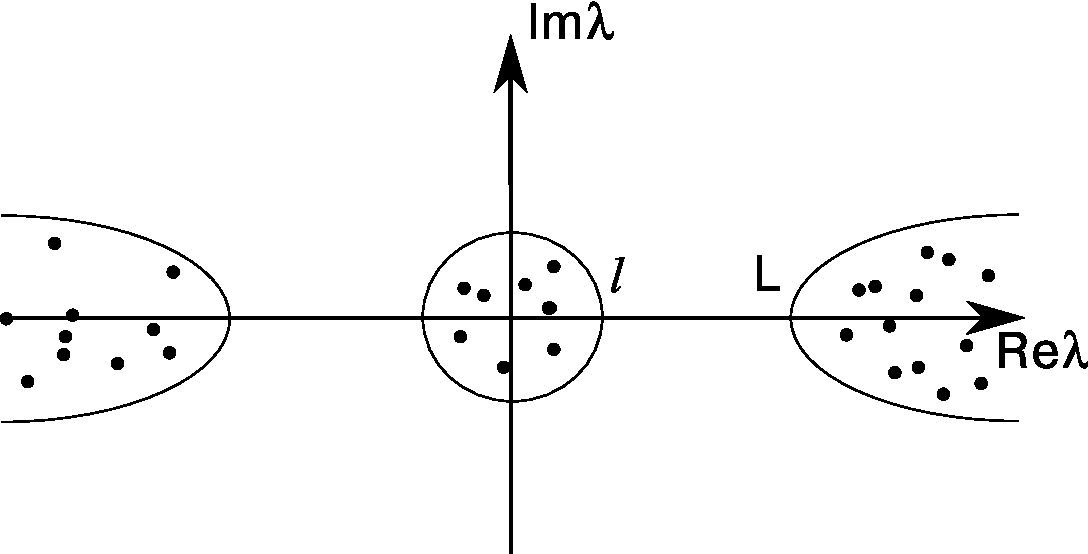
\includegraphics[height=0.45\textheight]{stiff.pdf}%
	\end{figure}
\end{frame}

\begin{frame}\frametitle{Спектр жесткой краевой задачи}
	Решение краевой задачи - некоторая линейная комбинация решений с различными $\lambda$, причем
	решения с $\lambda$ из
	\begin{itemize}
		\item мягкого спектра - небольшие по модулю
		\item жесткого положительного спектра - резко убывают влево
		\item жесткого отрицательного спектра - резко убывают вправо
	\end{itemize}
\end{frame}

\subsection{Вычислительная корректность}
\begin{frame}\frametitle{Граничные условия для жесткой краевой задачи}
	Пусть в жесткой отрицательной части спектра находится $I_-$ собственных значений, причем это число больше числа граничных условий слева $k$.
	Решения из жесткой отрицательной части спектра быстро убывают вправо, и на правом конце по модулю очень малы (в $e^{LT}$ раз меньше чем на левом).
	Из-за этого, их вклад в граничные уравнения на правом конце практически нулевой (порядка ошибок округления).

	Изменение коэффициентов при этих решениях практически не повлияет на правые граничные условия, поэтому коэффициенты можно надежно найти только из левых граничных
	условий. А левых граничных условий недостаточно, чтобы найти все коэффициенты при убывающих вправо решениях.
\end{frame}

\begin{frame}\frametitle{Необходимое условие корректности}
	Итак, чтобы задача была \emph{вычислительно корректной} требуется чтобы число условий слева было не меньше убывающих вправо решений, и, наоборот,
	число условий справа было не меньше числа убывающих влево решений.
\end{frame}

\begin{frame}[plain]
  \begin{center}
  {\Huge Спасибо за внимание!}
  \vspace{8ex}

  Цыбулин Иван

  e-mail: \colorhref{mailto:tsybulin@crec.mipt.ru}{tsybulin@crec.mipt.ru}
  \end{center}
\end{frame}

\end{document}
